\documentclass[BTech]{nitkdiss}

\usepackage{amsmath,amssymb,graphicx,color,colortbl}

\title{Perforator Evaluation using Hand-held Ultrasound Doppler Device}
\author{Pavan M (15EC137)\\ Pruthvik A (15EC139)\\ Vangala Rajiv Srivatsava (15EC248)\\}
\mentor{Dr. Deepu Vijayasenan}
\date{\today}
\department{Electronics and Communication Engineering}

\begin{document}

\maketitle

\newpage
\begin{abstract}

\hspace{0.4cm} The purpose of our project is to determine the physical dimensions, like diameter and depth from the skin, of  perforators, and its blood flow characteristics like velocity by Ultrasound Doppler examination.

Ultrasound Doppler uses high frequency sound waves to measure the amount of blood flow in blood vessels. It works on Doppler Effect phenomenon which changes the frequency depending on the relative motion of the observer and the object where the reflection of sound wave takes place. By studying the shift in frequency be will be able to calculate the motion of the object (in our case blood inside blood vessels). The ultrasound waves collide with the red blood cells and reflect back to the receiver of the hand held doppler. Our part in this project is to develope algorithms to analyze this reflected sound and to find the velocity, diameter and depth of the perforator.
\end{abstract}

\newpage
\tableofcontents
\listoffigures
\listoftables
\newpage
\pagestyle{plain}
\pagenumbering{arabic}

\chapter{Introduction}           

\section{ Problem definition } 
\hspace{0.4cm}Perforator veins are so called because they perforate the deep fascia of muscles, to connect the superficial veins to the deep veins where they drain. They drain away the excess blood from the superficial veins into deep veins. Hence they maintain correct blood draining. They have valves which prevent blood flowing back from deep to superficial veins in muscular systole or contraction.

\begin{center}
%\begin{figure}[h]
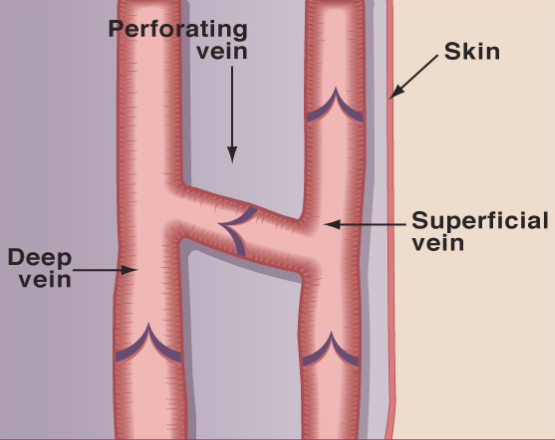
\includegraphics[scale = 0.40]{perforator.png}
\captionof{figure}{Perforator vein lateral view}
%\end{figure}
\end{center}




\hspace{0.4cm} Perforators play a vital role in providing regular blood supplies to the skin tissues. Hence, during Skin reconstructive surgeries it is very important to have a good knowledge of the physical characteristcs of the perforators supplying blood such as \\
1. Depth from skin\\
2. Diameter\\
and also the Velocity of blood within the perforator.

We need a non invasive technique to determine these. Reliability is also a matter of concern. Along with reliability the setup should be portable and cost effective compared to other existing non invasive techniques and informative too. Our aim is to derive all the information we require by analysing the sound recieved by a portable hand-held Ultrasound Doppler device and provide reliable output.



\section{Previous work}
\hspace{0.4cm} Imaging (colour) Ultrasound doppler technique has been extensively used to determine physical characteristics of the perforator. It gives all the desired output. But it comes with a draw back. Portability and cost is an issue. It can't be used in the operation theatre due to portabililty issue. So an alternative portable device non-imaging(hand-held) Ultrasound doppler is being used as an alternative. Output of this device is mere sound. So a trained ear can understand the physical characteristics. We need to develope a more reliable output from the device.

\begin{center}
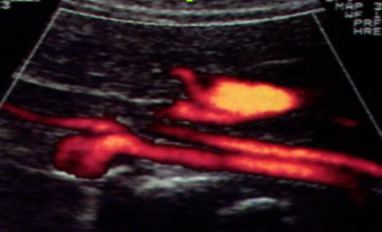
\includegraphics[scale = 0.6]{Colour_Doppler.png}
\captionof{figure}{Imaging (Colour) Doppler Image}
\end{center}


\begin{center}
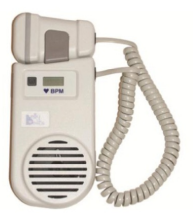
\includegraphics[scale = 0.7]{H_Doppler.png}
\captionof{figure}{Non Imaging (Hand-held) Doppler Device}
\end{center}




\section{Motivation}
\hspace{0.4cm} It is very important that during reconstructive surgery that the doctors have knowledge of the blood vessels and skin tissues (mainly perforators). Lack of availability of Imaging Ultrasound Doppler in the operation theatre forces us to use some portable device. So till now doctors listen to the output of the hand-held ultrasound doppler and based on their experience proceed with the surgeries. This is not a reliable practice. So we had to come up with algorithm to give us the write knowledge about the perforators. 

\section{Overview}          
\hspace{0.4cm} We know the importance of perforators for successful reconstructive surgeries. We cant afford to make mistakes in the algorithm. We are given audio samples, which is the Doppler frequency shift spectrum produced by moving red cells in the path of the ultrasound beam. We need to calculate the frequency shift by frequency analysis techniques and Calcuate the blood flow characteristics and physical characteristics of perforator arteries. Then we need to check our output with the standard output obtained from the Imaging (colour) Doppler and improvise on our algorithm to obtain output with maximum accuracy as possible. 

\chapter{Description}
\section{Evaluation of Perforator}
\hspace{0.4cm} Velocity, Depth and Diameter of the perforator can be determined by analysing some physical characteristics of sound like frequency, amplitude. 
\subsection{Velocity}
\hspace{0.4cm} Velocity can be analysed using doppler effect. The shift in frequency is directly proportional to the velocity of red blood cells within the perforator. \\

 { \Huge \[ \Delta f = \frac{2 * F_T * v * cos \theta}{C} \] }
 
 The above equation is derived from the Doppler effect frequency shift formula. where, $\Delta f = frequency shift$\\ $F_T = transmission frequency of hand-held doppler$\\ $v = velocity of blood in perforator$\\ $\theta = angle the incident sound wave makes with the perforator$\\ $C = speed of sound travelling in skin tissues$\\
 
\subsection{Depth}

\hspace{0.4cm} More the depth the perforator is situated from the skin softer is the sound. The loudness of the sound will reduce with the depth. Therefore the sound waves that is reflected from the perforators that are situated deep inside the skin with have lesser ampltidue compared to the that which is situated nearer to the skin. Depth increases with increase in the BMI (Body Mass Index) of the patient.


\subsection{Diameter}

\hspace{0.4cm} Sound reflected from the bigger diameter perforators will be louder with more bass i.e the sound will be flatter. Hence, the sound will have low frequencies compared to that of smaller diameter perforators.

\section{Sound Processing}

\hspace{0.4cm} For sound processing we have used python programming language. Another alternative available for us was Matlab. Though Matlab was more convenient because of the in built sound processing softwares we had to chose python.It is very easy to share code and anyone can make changes in the future and improvise the algorithm. Not everyone will be accessible to Matlab software. Some packages like scipy and numpy are very useful in sound processing applications. Combining it with Matplot library to plot graphs, python is very much comparable with Matlab software.

\chapter{Conclusions}

\hspace{0.4cm} We started with the evaluation of velocity. We tried few techniques to evaluate the doppler shift from the given samples. First one was by finding the Spectrogram of the sample.\\
\\
\hspace{0.4cm} A spectrogram is a visual representation of the spectrum of frequencies of sound or other signal as they vary with time. We determined the short time fourier transform of window length 25ms in order to study the fourier spectrum of each window over time and developed a spectrogram from it. The spectrogram gave as an idea on the periodicity of the high frequency shifts caused during Systole of the heart (which is periodic). 

\begin{center}
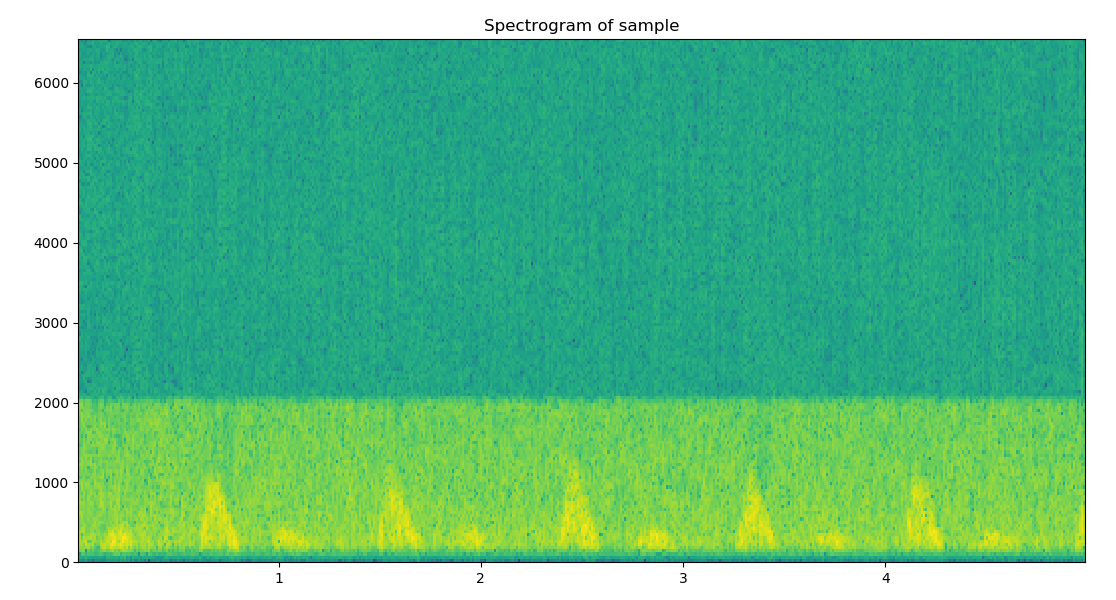
\includegraphics[scale = 0.4]{spec.png}
\captionof{figure}{Spectrogram of our sample ultrasound doppler}
\end{center}

\hspace{0.4cm} But with just the spectrogram we were able to clearly tell the frequency shift. As there was periodicity observed in the spectrogram, Auto-correlation would give us a better idea about the shift.
The difference between the middle peak and the first peak on the either side(symmetric) gave us the number frame shift.

\begin{center}
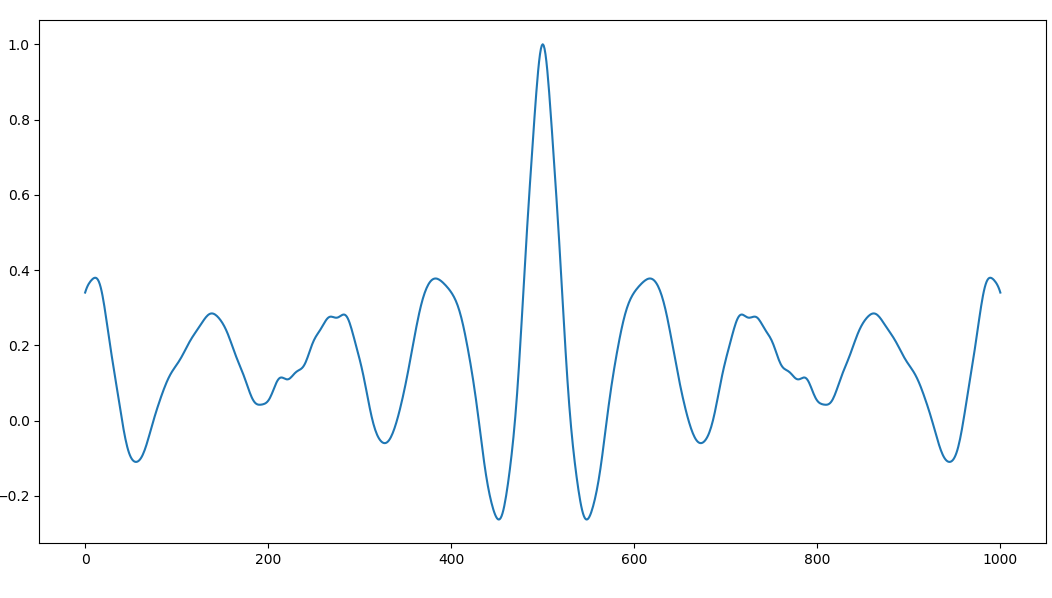
\includegraphics[scale = 0.33]{auto1.png}
\captionof{figure}{Auto-Correlation of one window (size 25ms) of our ultrasound doppler sample}
\end{center}
 

\section{Analysis}
\hspace{0.4cm} We did an auto correlation of a sample of window size of 25ms. We found the index of first peak after the 0th index peak (middle -largest). It gave us number of frame shifts. Frequency shift can be found out by dividing sample frequency by number of frame shifts. We drew a plot containing the the frame shift of each window over 100 windows. Then found out the minimum frame shift over 100 windows. Here finding minimum shift was essential because minimum shift gave us the maximum frequency shift hence maximum velocity as frequency shift and velocity is directly proportional to each other.

\begin{center}
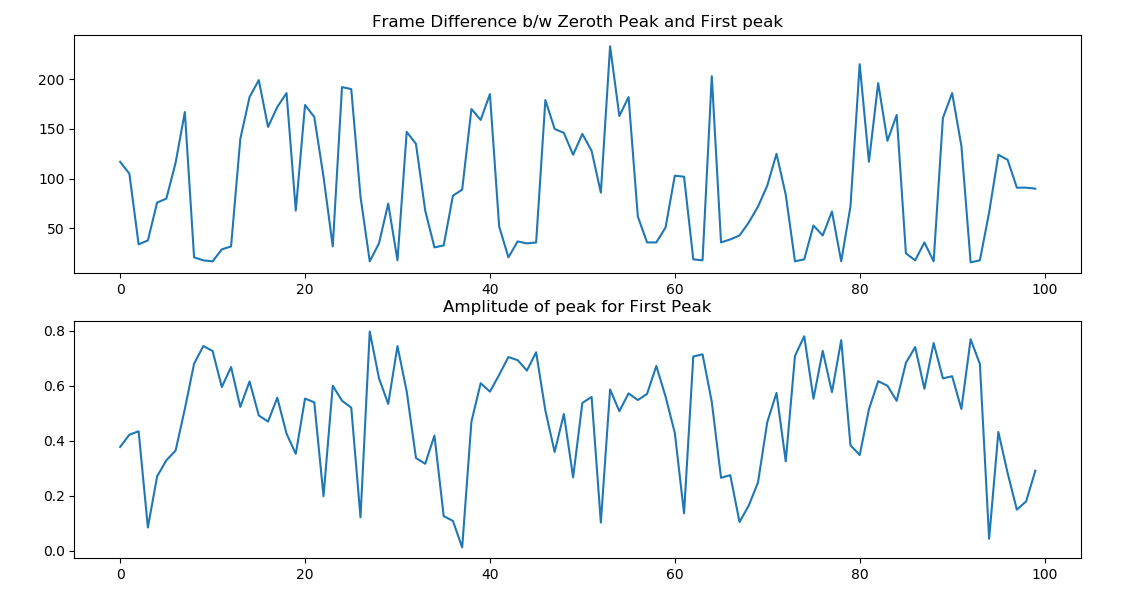
\includegraphics[scale = 0.33]{auto2.png}
\captionof{figure}{Frame Shifts of First Peak over 100 windows with corresponding Amplitude}
\end{center}

\hspace{0.4cm} By putting the value of the frequency shift in the formula,\\

\begin{equation}
\Delta f = \frac{2 * F_T * v * cos \theta}{C}
\end{equation}


And other values (in our case),

$\Delta f = 44100 / frame shift$,(44100 $=$ sampling frequency)
$F_T = 4.0 MHz$,
$\theta = 60\deg$,
$C = 1540 m/s$, we can estimate the velocity. 


\hspace{0.4cm} First we worked with dual channel data and we had to shift to single channel data because our primary aim was to record audio on phone and phone supports only single channel mic input. The noise component increased when we shifted to single channel data samples. Removing noise was our primary goal.\\

\begin{center}
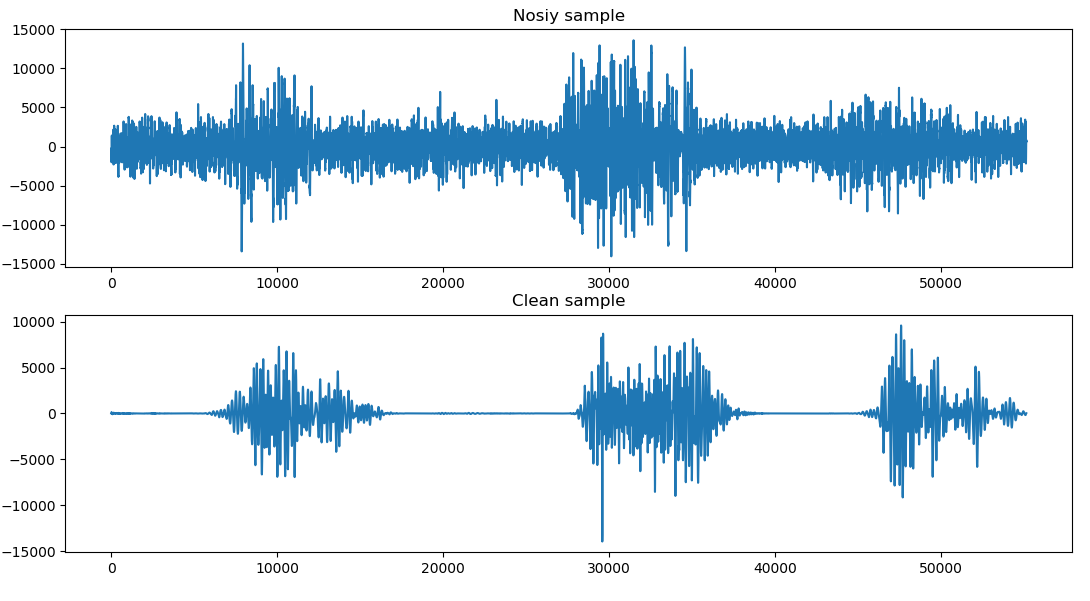
\includegraphics[scale = 0.4]{clean_noisy.png}
\captionof{figure}{Comparison between Nosiy and Clean data}
\end{center}

\begin{center}
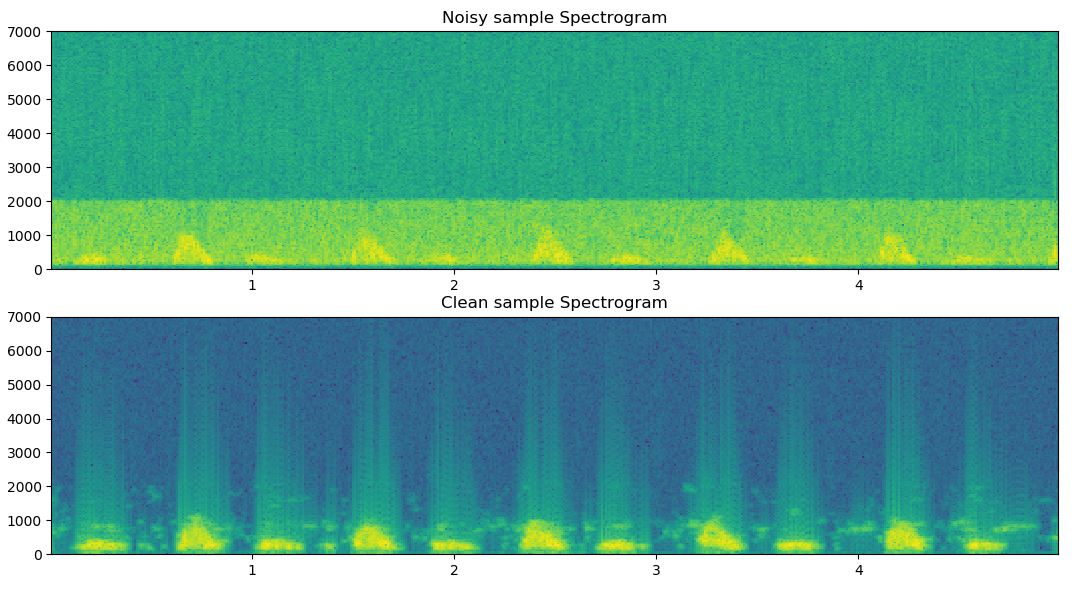
\includegraphics[scale = 0.4]{spec_cleanvsnoisy.png}
\captionof{figure}{Spectrogram Comparison between Nosiy and Clean data}
\end{center}

\hspace{0.4cm} The above graphs shows the comparison between Nosiy and clean data. The data was clean using Audacity software combined with wiener filter and band pass filter. \\

\hspace{0.4cm} Auto correlation on both the above samples gave similar results which was unexpected. This was due to higher frequency components by noise during non systole or diastole regions. Therefore, we have to isolate those regions. We had to implement our algorithm only during systole and diastole region. We proceeded with extracting the peak value from spectrogram.\\

\begin{center}
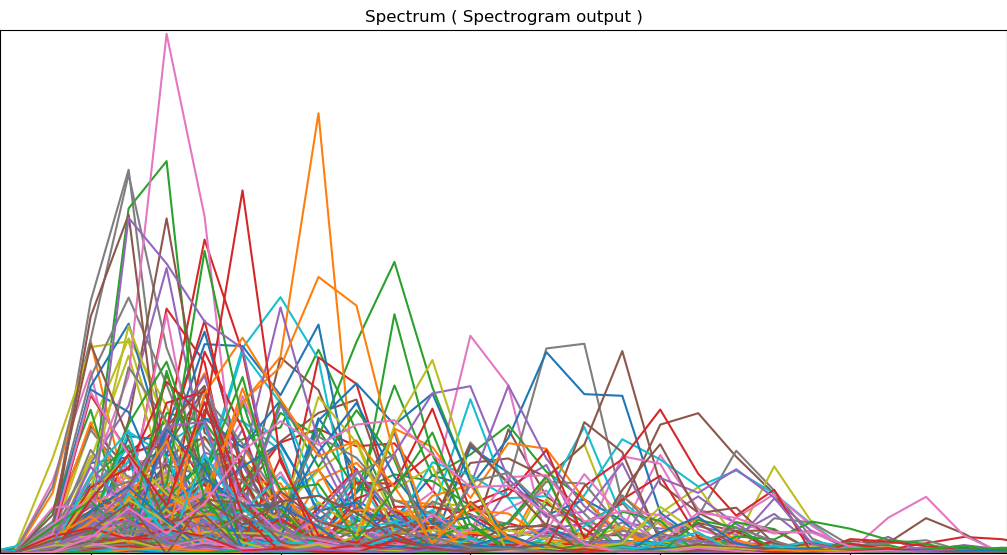
\includegraphics[scale = 0.36]{spectrum.png}
\captionof{figure}{Spectrum analysis of sample}
\end{center}

\hspace{0.4cm} There were many frequency components in spectrum. And the maximum amplitude did not correspond to maximum frequency component. So extracting maximum frequency component from this spectrum is difficult, so we had to stick with auto correlation.

\begin{center}
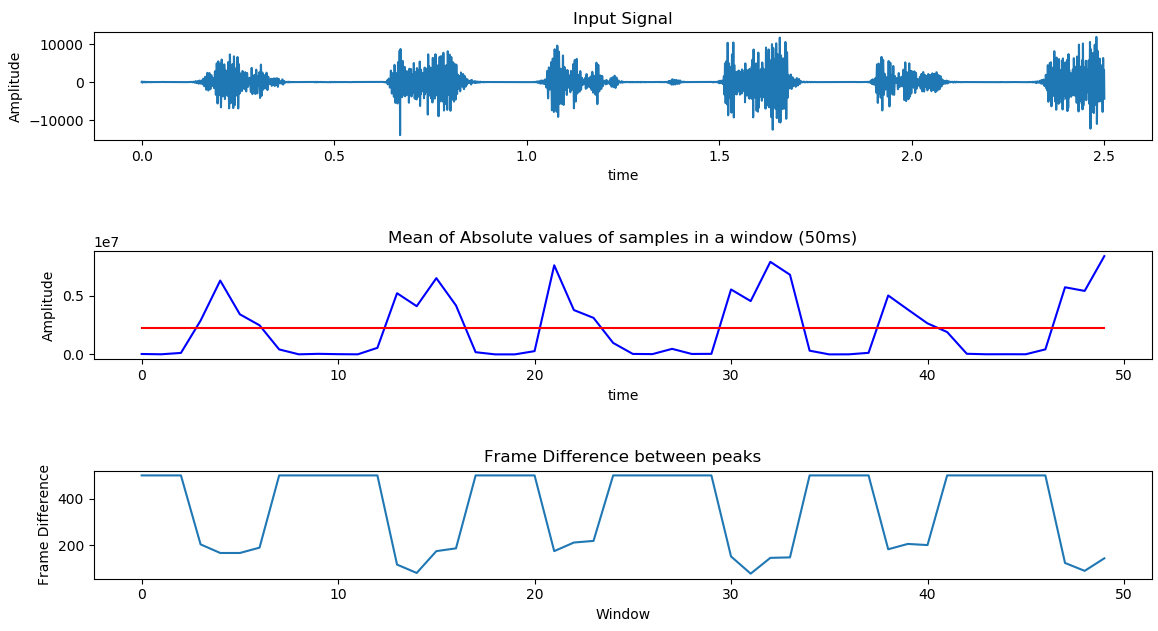
\includegraphics[scale = 0.38]{clean_auto.png}
\captionof{figure}{Auto Correlation only during peaks (Clean sample)}
\end{center}



\begin{center}
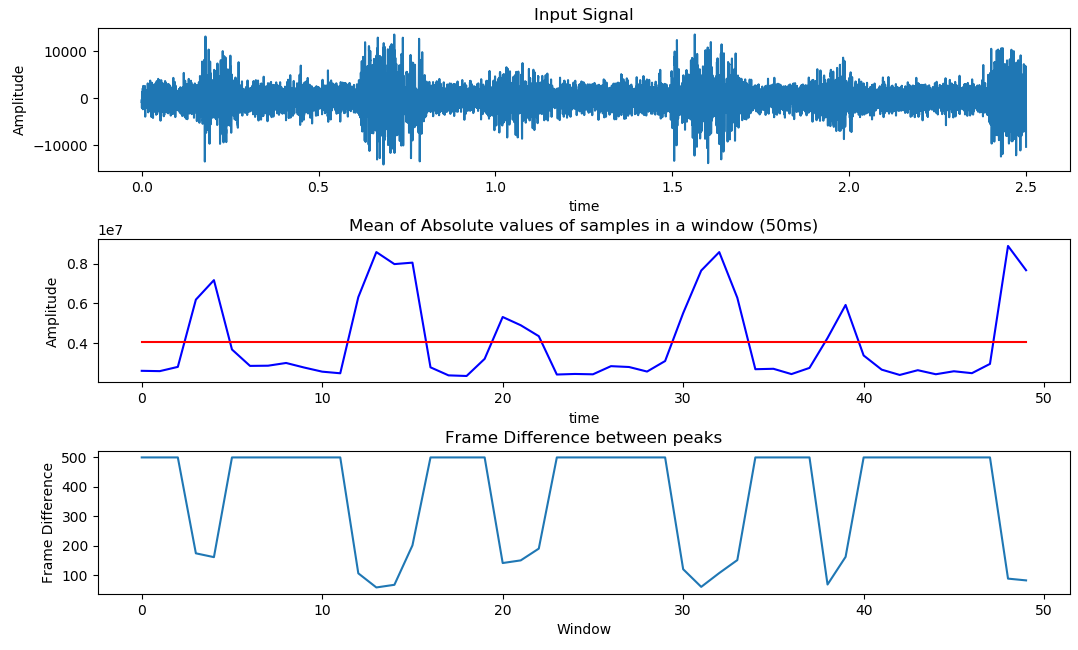
\includegraphics[scale = 0.38]{noisy_auto.png}
\captionof{figure}{Spectrum analysis of sample}
\end{center}

\hspace{0.4cm} Window size of 50ms of the sample was taken and mean of absolute values of the samples within that window was taken. If the mean of the window is greater than the mean of the whole sample then that window was considered for auto correlation. For clean data we got values very close to the expected value ( percentage error less than 5\%)

\hspace{0.4cm} When an unclean sample was used then the percentage error was around 10\%. Below table includes 4 samples' clean versus unclean data comparison of our velocity estimation. \\


\begin {table}
\caption {Observed Velocity over different samples}
\begin{center}
 \begin{tabular}{||c| c| c| c||} 
 \hline
 Sample Number & Expected Velocity & Clean data & Unclean Data \\ [0.5ex] 
 \hline\hline
 1 & 22 & 22.05 & 29.27 \\ 
 \hline
 2 & 15 & 12.78 & 17.04 \\
 \hline
 3 & 22 & 21.12 & 25.34 \\
 \hline
 4 & 15 & 13.14 & 16.89 \\ [1ex] 
 \hline
\end{tabular}
\end{center}
\end{table}

\hspace{0.4cm} To reduce the noise we implemented wiener filter. The percentage error reduced to some extent.\\

Gain of Wiener filter is given by, \\
\begin{equation}
G(K) = \frac{1}{1 + \frac{S_n(K)}{S_x(K)-S_n(K)}}
\end{equation}

where,

$S_n(K) = || N(k) ||^2 $ ( average of square of samples in non peak windows ) \\
$S_x(K) = || X(k) ||^2 $ ( average of square of samples in peak windows )\\

\begin{equation}
Wiener Output = S(K) * G(K)
\end{equation}

\begin{center}
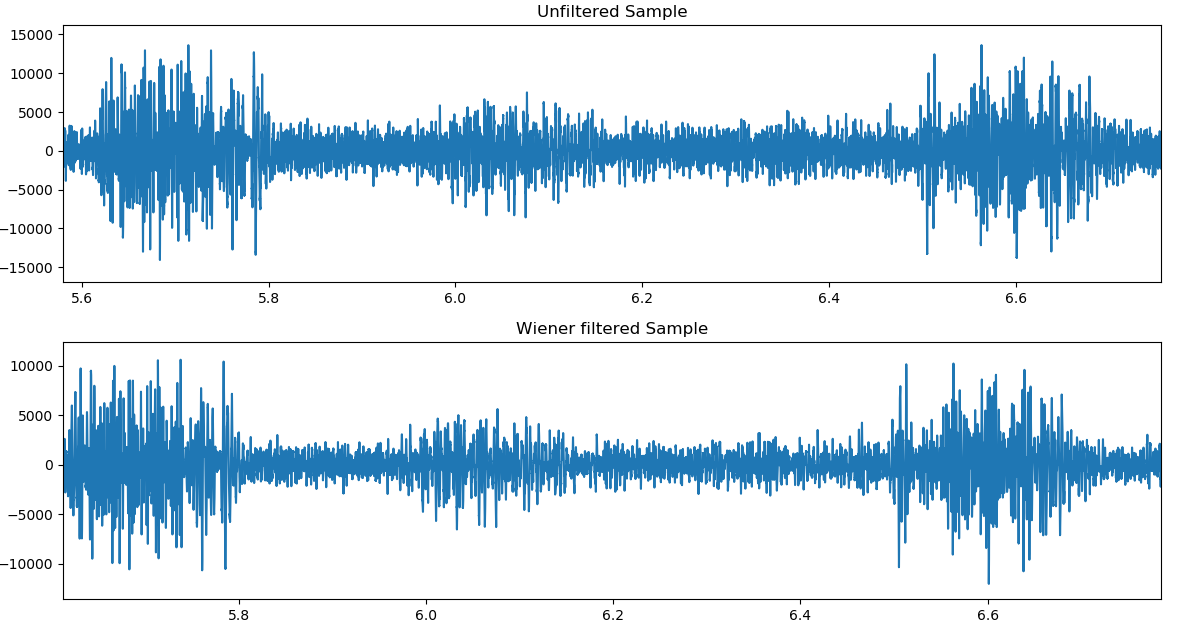
\includegraphics[scale = 0.4]{wiener.png}
\captionof{figure}{Wiener filtered sample}
\end{center}


\begin {table}
\caption {Observed Velocity of Unfiltered and wiener filtered Data}
\begin{center}
 \begin{tabular}{||c| c| c| c||} 
 \hline
 Sample Number & Expected Velocity & Wiener filtered data &  Unfiltered Data \\ [0.5ex] 
 \hline\hline
 1 & 22 & 26.41 & 29.27 \\ 
 \hline
 2 & 15 & 16.67 & 17.04 \\
 \hline
 3 & 22 & 21.12 & 25.34 \\
 \hline
 4 & 15 & 13.14 & 13.14 \\ [1ex] 
 \hline
\end{tabular}
\end{center}
\end{table}


\hspace{0.4cm} There is very slight reduction is noise not to the extent we desired. The percentage error came down by a slight margin after looking into the table.


\section{Future Work}

\begin{itemize}
\item Wiener filter has to be improved.
\item Need to develope algorithm to find Depth of the perforator from the skin.
\item Need to develope algorithm to find Diameter of the perforator.
\item Need to make the developed algorithm available on a portable device like mobile.
\end{itemize}


\begin{thebibliography}{9}

%\begin{enumerate}
\item Milton SH. Pedicled skin-flaps: the fallacy of the length:width ratio.B J Surg 1970;57:502-8.
\item Taylor GI, Palmer JH. The vascular territories (angiosomes) of the body: experimental study and clinical applications. Br J Plast Surg 1987; 40:113-41.
\item Phd Thesis on studying the physical characteristics of the sound produced by the blood flowing through the leg arterial perforator vessels, by using acoustic hand held Doppler and colour Doppler.
%\end{enumerate}

\end{thebibliography}

\end{document}
